\noindent
\begin{tcolorbox}[colframe=black,width =7cm,colback=gray!20,arc=0pt]
\centering {\sc {\bf Questão 02}}
\end{tcolorbox}

Considere os sinais
\begin{align*}
    x_{AR}(n) &= -0.8987 x(n-1) –0.9018 x(n-2) + \nu(n) \\
    x_{ARMA}(n) &= 1.9368 x(n-1) –0.9519 x(n-2) + \nu(n) –1.8894 \nu(n-1) + \nu(n-2)
\end{align*}

\begin{enumerate}[label={\bf \alph*:},series=exerc,align=left]
    \item \textbf{Obtenha e trace a densidade espectral de potência de ambos os sinais.}

    Para cada item, podemos transformar as equações a diferenças em suas respectivas funções de transferência:
    \begin{align*}
        X_{AR}(z) &= \frac{A_{AR}(z)}{B_{AR}(z)} = \frac{1}{1+0.8987z^{-1}+0.9018z^{-2}}N(z) \\
        X_{ARMA}(z) &= \frac{A_{ARMA}(z)}{B_{ARMA}(z)} = \frac{1-1.8894z^{-1}+z^{-2}}{1-1.9368z^{-1}+0.9519z^{-2}}N(z)
    \end{align*}

    Como sabemos a relação entre a densidade espectral de potência e as expressões $A(z)$ e $B(z)$, temos, supondo que o ruído tem variância unitária:

    \begin{align*}
        \phi_{AR}(z) &= \frac{A_{AR}(z)A^*_{AR}(\frac{1}{z^*})}{B_{AR}(z)B^*_{AR}(\frac{1}{z^*})} = \frac{1}{\left(1 + \frac{0.8987}{z} + \frac{0.9018}{z^{2}}\right) \left(0.9018 z^{2} + 0.8987 z + 1\right)} \\
        \phi_{ARMA}(z) &= \frac{A_{ARMA}(z)A^*_{ARMA}(\frac{1}{z^*})}{B_{ARMA}(z)B^*_{ARMA}(\frac{1}{z^*})} = \frac{\left(1.0 - \frac{1.89}{z} + \frac{1}{z^{2}}\right) \left(z^{2} - 1.89 z + 1.0\right)}{\left(1.0 - \frac{1.94}{z} + \frac{0.952}{z^{2}}\right) \left(0.952 z^{2} - 1.94 z + 1.0\right)}
    \end{align*}
    Lembrando que podemos fazer a substituição $z=e^{i\omega}$, podemos plotar as funções $\phi(\omega)$:

    \begin{figure}[h!]
        \centering
        \begin{subfigure}{0.4\textwidth}
            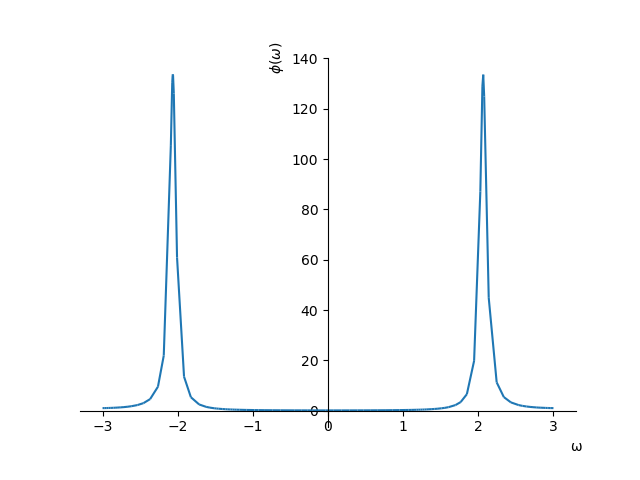
\includegraphics[width=\textwidth]{../img/02/PSD_AR}
            \caption{Modelo AR}
        \end{subfigure}
        \begin{subfigure}{0.4\textwidth}
            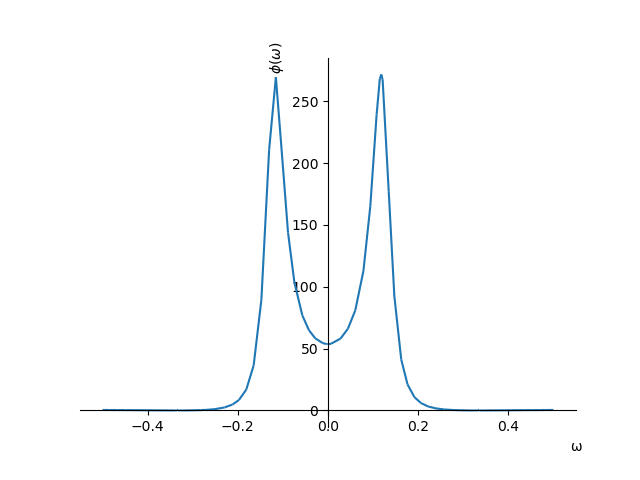
\includegraphics[width=\textwidth]{../img/02/PSD_ARMA}
            \caption{Modelo ARMA}
        \end{subfigure}
    \end{figure}

    \item \textbf{Considere, para cada um deles, uma realização com um número suficiente de dados, e forneça a densidade espectral de potência a partir da transformada de Fourier de uma estimação temporal da autocorrelação.}

    Podemos simular estes experimentos amostrando um número suficientemente grande de ruído, independente, gaussiano, de média nula e variância unitária e submetendo-o ás funções de transferência acima.
    A partir do cálculo do vetor de autocorrelação podemos estimar a densidade espectral de potência com sua Transformada de Fourier.
    Para ambos os casos foram amostrados $1000$ pontos e calculado o vetor de autocorrelação até um lag de $500$ unidades.

    \begin{figure}[h!]
        \centering
        \begin{subfigure}{0.4\textwidth}
            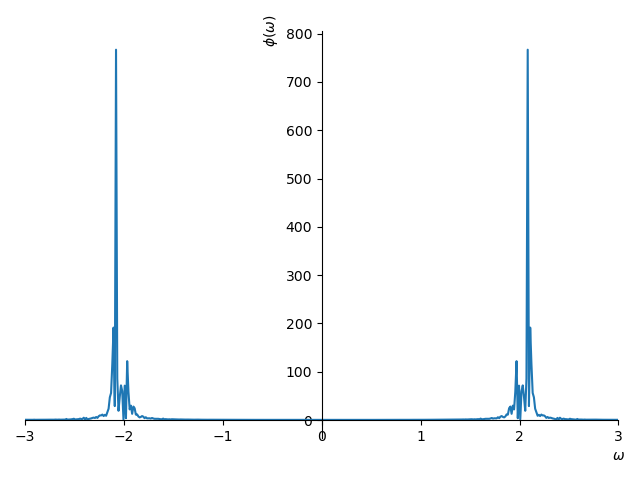
\includegraphics[width=\textwidth]{../img/02/PSD_AR_simulated}
            \caption{Modelo AR}
        \end{subfigure}
        \begin{subfigure}{0.4\textwidth}
            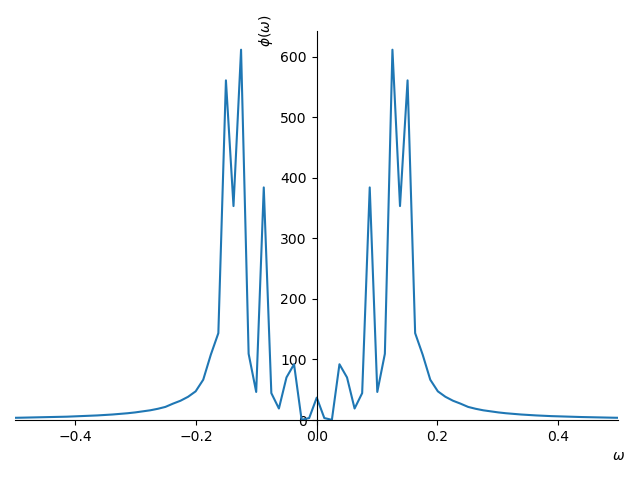
\includegraphics[width=\textwidth]{../img/02/PSD_ARMA_simulated}
            \caption{Modelo ARMA}
        \end{subfigure}
    \end{figure}

    Podemos observar que os gráficos obtidos se aproximam muito bem dos teóricos, apresentados anteriormente.
\end{enumerate}
